\documentclass[a4paper]{article}
\usepackage{amsmath}
\usepackage{fancybox}
\usepackage{amssymb}
\usepackage{capt-of}
\usepackage{pgfplots}
\usepackage{tikz}
\usetikzlibrary{matrix}
\usetikzlibrary{calc}
\usetikzlibrary{patterns}
\usetikzlibrary{decorations.pathreplacing}
%\tikzset{
%	CE/.style={column #1/.style={nodes={text width=24mm}}}
%}
%\tikzset{
%	CA/.style={column #1/.style={nodes={text width=35mm}}}
%}
\tikzset{
	CE/.style={column #1/.style={nodes={text width=25mm}}}
}
\tikzset{
	CA/.style={column #1/.style={nodes={text width=36mm}}}
}
\begin{document}
\begin{tikzpicture}[scale=1.5][master]
	\begin{axis}[enlargelimits=0.1,]
		\addplot+ [nodes near coords,only marks,point meta=explicit symbolic]
		table [meta=label] {
			x    y   label
			1  -1  $u_{1}$
			2  -1.666 $u_{2}$
			3  -2 $u_{3}$
			4  -2.2  $u_{4}$
			5  -2.333 $u_{5}$
			6  -2.428 $u_{6}$
			7  -2.5 $u_{7}$
			8  -2.555 $u_{8}$
			9  -2.6 $u_{9}$
		};
	\end{axis}
\end{tikzpicture}

\begin{tikzpicture}[>=latex]
	\begin{axis}[
		axis x line=center,
		axis y line=center,
		xtick={-5,-4,...,5},
		ytick={-5,-4,...,5},
		xlabel={$x$},
		ylabel={$y$},
		xlabel style={below right},
		ylabel style={above left},
		xmin=-5.5,
		xmax=5.5,
		ymin=-5.5,
		ymax=5.5]
		\addplot[domain=-1:1] {-2*(\x)^2+2};
		\addplot[domain=1:3] {2*(\x)-3};
		\addplot[mark=*] coordinates {(3,3)};
		\addplot[mark=*,fill=white] coordinates {(1,-1)};
		\addplot[mark=*,fill=white] coordinates {(-1,0)};
		\addplot[mark=*] coordinates {(1,0)};
	\end{axis}
\end{tikzpicture}

\[\textbf{$\left(x\right)\left(2x^2+3x-2\right)\leq 0$}\]


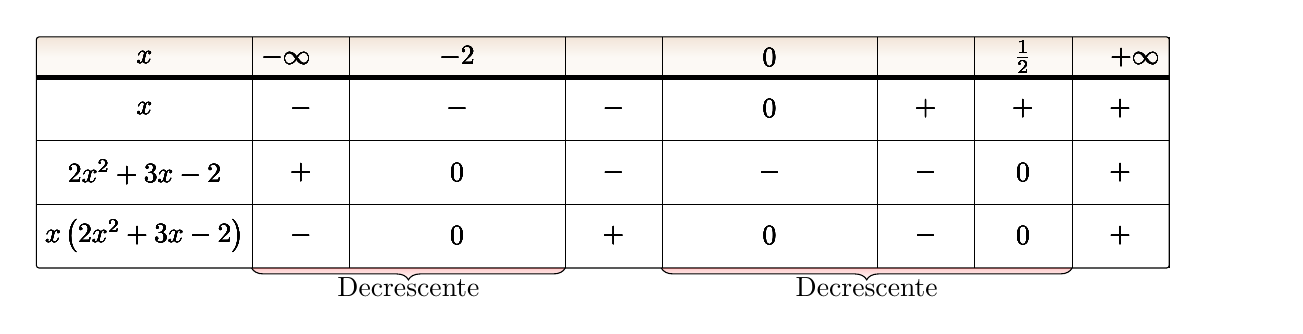
\begin{tikzpicture}
		%\matrix[matrix of math nodes,
		%nodes in empty cells,
		%nodes={text width=2cm,minimum height=8mm,anchor=north east, text centered}, 
		%row 1/.style={nodes={minimum height=5mm}},CE/.list={1,3,5}](S)
		\matrix[matrix of math nodes,
		nodes in empty cells,
		nodes={text width=1cm,minimum height=8mm,anchor=north east, text centered}, 
		row 1/.style={nodes={minimum height=5mm}},CE/.list={1,3,5}](S)
		{
			& & & & & & & & \\
			& & & & & & & & \\
			& & & & & & & & \\
			& & & & & & & & \\
		};
		\fill[top color=brown!20,bottom color=brown!5,middle color=brown!5](S-1-1.south west) [rounded corners=1pt] |- (S-1-8.north east) |- cycle;
		\draw[rounded corners=1pt] (S-1-1.north west) rectangle (S-4-8.south east);
		\draw[ultra thick] (S-1-1.south west) -- (S-1-8.south east);
		\draw (S-2-1.south west) -- (S-2-8.south east);
		\draw (S-3-1.south west) -- (S-3-8.south east);
		\foreach \i in{1,...,8}{
			\draw (S-1-\i.north east) -- (S-4-\i.south east);
			\node at (S-1-1) {$x$};
			\node[anchor=west] at (S-1-2.west) {\(-\infty\)};
			\node[anchor=east] at (S-1-8.east) {\(+\infty\)};
			\node at (S-1-3) {\(-2\)};
			\node at (S-1-5) {\(0\)};
			\node at (S-1-7) {\(\frac{1}{2}\)};
			\node at (S-2-1) {\(x\)};
			\node at (S-3-1) {\(2x^2+3x-2\)};
			\node at (S-2-2) {\(-\)};
			\node at (S-3-2) {\(+\)};
			\node at (S-2-3) {\(-\)};
			\node at (S-3-3) {\(0\)};
			\node at (S-2-4) {\(-\)};
			\node at (S-3-4) {\(-\)};
			\node at (S-2-5) {\(0\)};
			\node at (S-3-5) {\(-\)};
			\node at (S-2-6) {\(+\)};
			\node at (S-2-7) {\(+\)};
			\node at (S-2-8) {\(+\)};
			\node at (S-3-6) {\(-\)};
			\node at (S-3-7) {\(0\)};
			\node at (S-3-8) {\(+\)};
			\node at (S-4-1) {\(x\left(2x^2+3x-2\right)\)};
			\node at (S-4-2) {\(-\)};
			\node at (S-4-3) {\(0\)};
			\node at (S-4-4) {\(+\)};
			\node at (S-4-5) {\(0\)};
			\node at (S-4-6) {\(-\)};
			\node at (S-4-7) {\(0\)};
			\node at (S-4-8) {\(+\)};
		}
	\draw[top color=red, fill opacity=.2, decorate,decoration={brace,mirror,amplitude=1.5mm}](S-4-2.south west) to node[midway,fill opacity=1,below]{Decrescente} (S-4-3.south east);
	\draw[top color=red, fill opacity=.2, decorate,decoration={brace,mirror,amplitude=1.5mm}](S-4-5.south west) to node[midway,fill opacity=1,below]{Decrescente} (S-4-7.south east);
	\end{tikzpicture}

\[\textbf{C.S = $]-\infty,-2]\cup [0,\frac{1}{2}]$}\]
\[\textbf{$\left(x-2\right)\left(x^2+3\right)\left(4-x\right)>0$}\]


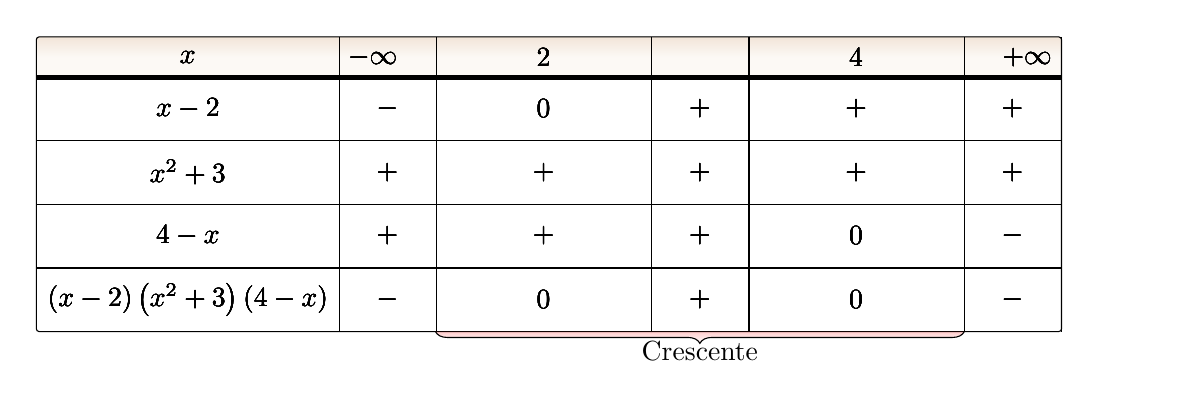
\begin{tikzpicture}
	%\matrix[matrix of math nodes,
	%nodes in empty cells,
	%nodes={text width=2cm,minimum height=8mm,anchor=north east, text centered}, 
	%row 1/.style={nodes={minimum height=5mm}},CE/.list={3,5},CA/.list={1}](S)
	\matrix[matrix of math nodes,
	nodes in empty cells,
	nodes={text width=1cm,minimum height=8mm,anchor=north east, text centered}, 
	row 1/.style={nodes={minimum height=5mm}},CE/.list={1,3,5},CA/.list={1}](S)
	{
		& & & & & & \\
		& & & & & & \\
		& & & & & & \\
		& & & & & & \\
		& & & & & & \\
	};
	\fill[top color=brown!20,bottom color=brown!5,middle color=brown!5](S-1-1.south west) [rounded corners=1pt] |- (S-1-6.north east) |- cycle;
	\draw[rounded corners=1pt] (S-1-1.north west) rectangle (S-5-6.south east);
	\draw[ultra thick] (S-1-1.south west) -- (S-1-6.south east);
	\draw (S-2-1.south west) -- (S-2-6.south east);
	\draw (S-3-1.south west) -- (S-3-6.south east);
	\draw (S-4-1.south west) -- (S-4-6.south east);
	\foreach \i in{1,...,6}{
		\draw (S-1-\i.north east) -- (S-5-\i.south east);
		\node at (S-1-1) {\(x\)};
		\node at (S-2-1) {\(x-2\)};
		\node at (S-3-1) {\(x^2+3\)};
		\node at (S-4-1) {\(4-x\)};
		\node at (S-5-1) {\(\left(x-2\right)\left(x^2+3\right)\left(4-x\right)\)};
		\node[anchor=west] at (S-1-2.west) {\(-\infty\)};
		\node[anchor=east] at (S-1-6.east) {\(+\infty\)};
		\node at (S-1-3) {\(2\)};
		\node at (S-1-5) {\(4\)};
		\node at (S-2-2) {\(-\)};
		\node at (S-2-3) {\(0\)};
		\node at (S-2-4) {\(+\)};
		\node at (S-2-5) {\(+\)};
		\node at (S-2-6) {\(+\)};
		\node at (S-3-2) {\(+\)};
		\node at (S-3-3) {\(+\)};
		\node at (S-3-4) {\(+\)};
		\node at (S-3-5) {\(+\)};
		\node at (S-3-6) {\(+\)};
		\node at (S-4-2) {\(+\)};
		\node at (S-4-3) {\(+\)};
		\node at (S-4-4) {\(+\)};
		\node at (S-4-5) {\(0\)};
		\node at (S-4-6) {\(-\)};
		\node at (S-5-2) {\(-\)};
		\node at (S-5-3) {\(0\)};
		\node at (S-5-4) {\(+\)};
		\node at (S-5-5) {\(0\)};
		\node at (S-5-6) {\(-\)};
	}
	\draw[top color=red, fill opacity=.2, decorate,decoration={brace,mirror,amplitude=1.5mm}](S-5-3.south west) to node[midway,fill opacity=1,below]{Crescente} (S-5-5.south east);
\end{tikzpicture}
\[\textbf{C.S = $]2,4[$}\]
	
	\begin{tikzpicture}[declare function={
			parabola(\x) = 2*\x-\x^2;
		}]
	  	\textbf{$2x-x^2 \geq 0 $}
		\begin{axis}[
			y axis line style={opacity=0},
			axis x line=middle,
			domain=-2:4,
			scaled ticks=false,
			ytick={\empty},
			xtick={\empty}, 
			xmin = -2,
			xmax = 4,
			ymin = -2,
			ymax = 2,
			]
			\addplot[no marks] {parabola(x)};
		\end{axis}
	    \node at (5.9,2){$-$};
	    \node at (5,2.5){$2$};
	    \node at (1,2){$-$};
	    \node at (1.8,2.5){$0$};
	    \node at (3.4,3.4){$+$};
	
	\end{tikzpicture}

\[\textbf{C.S = $[0,2]$}\]
\end{document}